% !TEX root = ../svrhm.tex
\section{Experiments}
\subsection{Experiment design}
%Architektur, Inputs, Outputs, Beschreibung Lernen der Koordinaten->Pixelwert Zuordnung, Lossfunktion
%Referenz zu analogem Experiment in FFM Paper
Using a similar experiment setup as described in \cite{tancik2020fourier}, we analyse the impact of applying population coding on the input of a neural network by training the network on a single image. 
It takes the image coordinates as inputs and performs a regression on the corresponding color values. 
We use a multilayer perceptron (MLP) with four hidden layers, each of size 256, and ReLU activations. 
The output consists of 3 channels with sigmoid activations for the RGB-values. 
The Mean Squared Error (MSE) is used as loss function. 
The input image consists of 12000 pixels of which 90\% are used as training data and 10\% as test data. 
The MLP is trained over 12000 epochs.

The input coordinates are scaled to $[-1,1]$. Five different population sizes $d \in \{16, 32, 64, 128, 256\}$ are examined. The network's output images are evaluated visually as well as quantitatively by the MSE.

\begin{figure}[h]
  \begin{minipage}{.48\textwidth}
    \centering
    \subcaptionbox{Input image\label{input}}
    {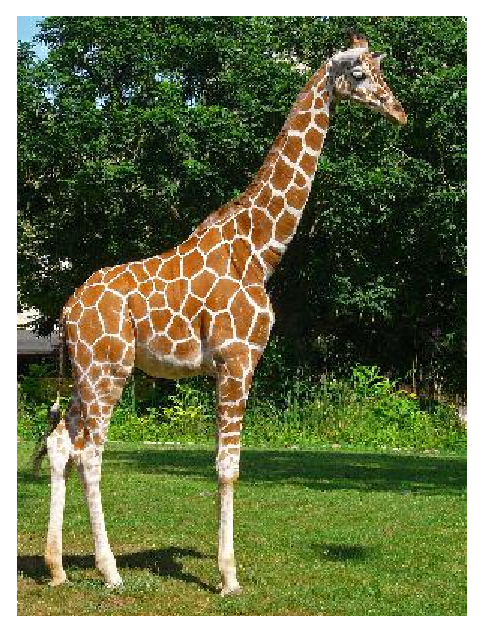
\includegraphics[width=0.45\textwidth]{Bilder/Giraffe/Giraffe_verkleinert_400x300.eps}}
    %\label{input}
    \subcaptionbox{No encoding\label{noEnc}}
    {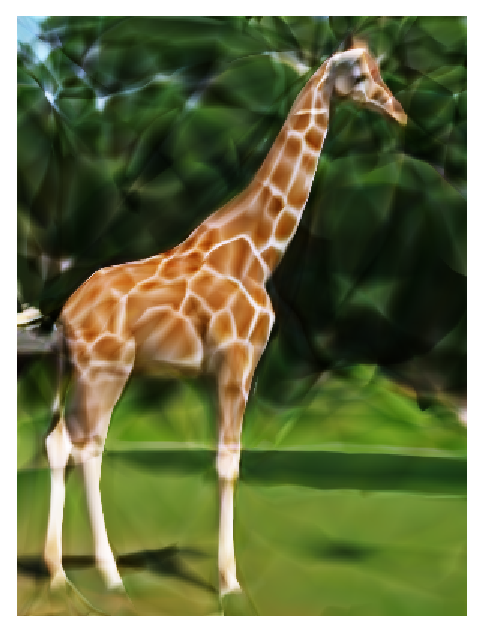
\includegraphics[width=0.45\textwidth]{Bilder/Giraffe/image_result_scale12000_indim2_lr0.003333.eps}}
      %\label{noEnc}
\caption{Reference image \cite{giraffeonline} and reconstructed image without encoding}
\label{InputNoEnc}
\end{minipage}\quad
\begin{minipage}[c]{.25\textwidth}
  \centering
  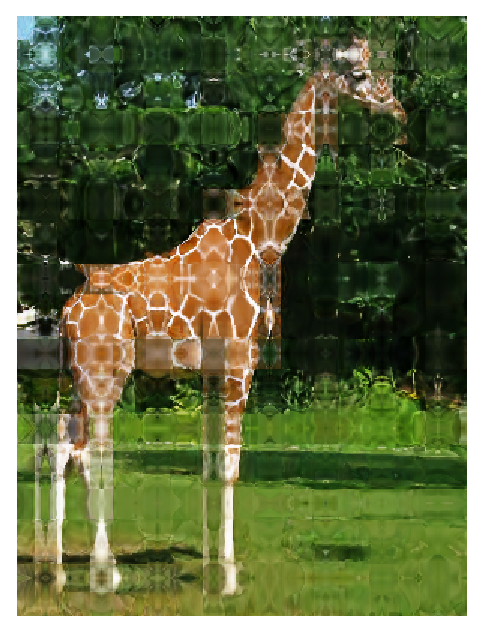
\includegraphics[width=\textwidth]{Bilder/Giraffe/spiegelungen_image_result_tent12000_indim16_lr0.0125_m5.eps}
  \caption{TE artifacts, $d$=16, $m$=5}
  \label{TEartefact}
\end{minipage}

\end{figure}


\begin{table}
  \caption{Minimum training and test loss achieved within 12000 epochs of learning for different encodings with dimension $d$.}
  \label{train_test_losses}
  \vspace{0.2cm}
  \centering
  \begin{tabular}[H]{cccc}
    \toprule
  \textbf{encoding} & $\boldsymbol{d}$ &\textbf{train loss} &\textbf{test loss}\\
  \midrule
  \textbf{none} & 2 & 0.016 & 0.018 \\
  \midrule
  \multirow{2}{*}{\textbf{FFM}} & 16 & 0.0086 & 0.0160 \\
    & 256 & 0.0057 & 0.0153 \\
  \midrule
  \multirow{2}{*}{\textbf{PE}} & 16 & 0.0063 & 0.0156 \\
  & 256 & 0.0004 & 0.0298 \\
  \midrule
  \multirow{2}{*}{\textbf{TE}} & 16 & 0.0092 & 0.0156 \\
    & 256 & 0.0005 & 0.0177 \\
  \midrule
  \multirow{2}{*}{\textbf{ME}} & 16 & 0.0111 & 0.0158 \\
  & 256 & 0.0007 & 0.0170 \\
  \bottomrule
  \end{tabular}
\end{table}

\begin{figure}
  \begin{subfigure}{0.5\textwidth}
    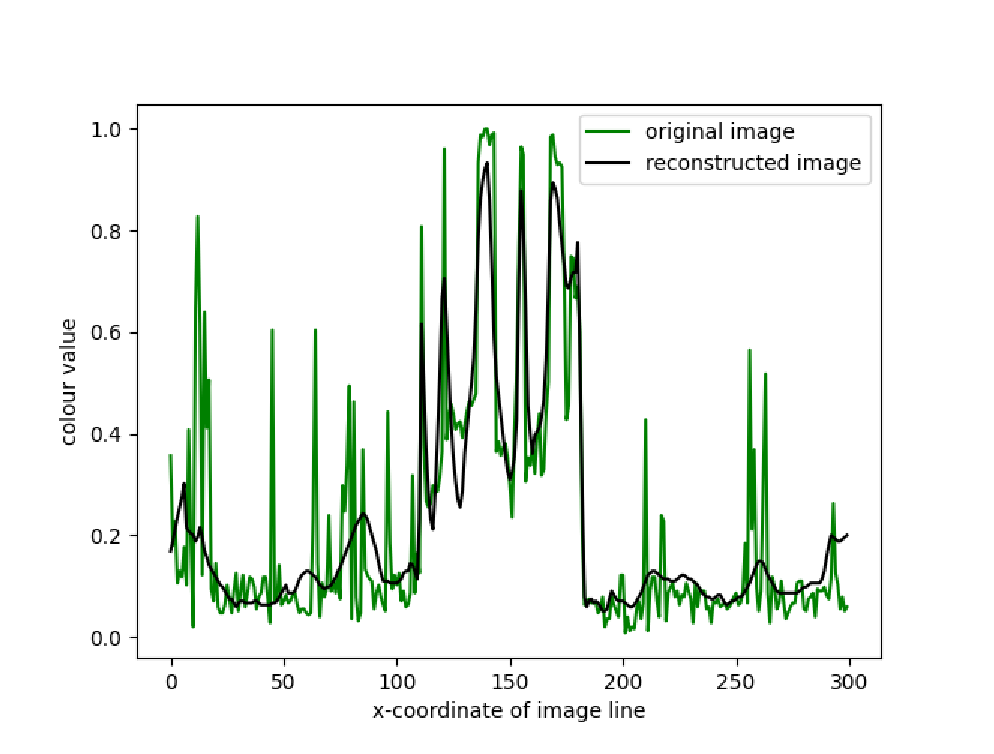
\includegraphics[width=.85\textwidth]{Bilder/Zeilenanalyse/lines_scale_channel1.eps}
   \end{subfigure}
   \begin{subfigure}{0.5\textwidth}
  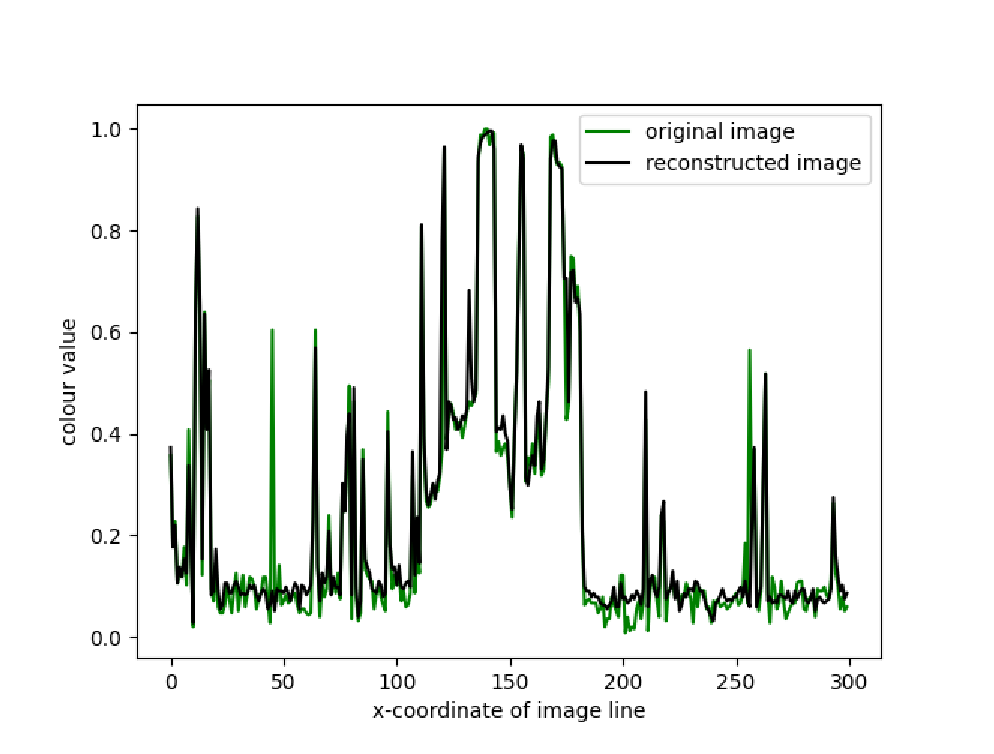
\includegraphics[width=.85\textwidth]{Bilder/Zeilenanalyse/lines_tent_channel1.eps}
  \end{subfigure}
  \caption{Values of green channel in row 150, top: no encoding, bottom: TE.}
  \label{lineAnalysis}
  % \caption{Reference image \cite{giraffeonline}, its reconstruction by an MLP without input encoding and a failed reconstruction with TE}
  % \label{RefNoEncTE}
\end{figure}

\subsection{Encodings}
In figure \ref{outputImages} the output images are visualized for each encoding. By only passing the two-dimensional coordinates as input, the MLP is unable to learn high-frequency dependencies (figure \ref{noEnc}). 
%The lowest train loss which is achieved within the 12000 epochs is $0.0159$ and the lowest test loss $0.018$. 
The utilisation of each encoding leads to higher resolution of the output. Using any encoding with population size $d = 16$ already yields a significant improvement in the reconstructed image. Increasing the population size enhances the output's image quality further. Population sizes beyond $d = 256$ offer diminishing returns. When using TE, the best results are achieved when setting $m$ to a quarter of the input dimension. Here, the output image of $d = 256$ with $m = 64$ can hardly be distinguished from the input image. Comparable results are achieved with ME and $d = 256$. 

In table \ref{train_test_losses}, the minimum training and test loss are shown. The results correlate with the visual observations. The use of each encoding, even with only 16 dimensions, leads to lower training losses. Notably, the test loss with $d=16$ in each encoding is better than the training loss with no encoding.

%Starting with $d = 16$, an improvement of the learning ability of the MLP can be observed. By the increase of $d$, the MLP performs better.


\begin{figure}[!h]
    
    \begin{subfigure}{.25\textwidth}
      
\includegraphics[width=\textwidth]{Bilder/Giraffe/Bildausschnitte/image_result_fourier12000_indim16_lr0.0125.eps}
      \caption{FFM, $d$=16}
      \label{FFM16}
    \end{subfigure}\hfil
    \begin{subfigure}{.25\textwidth}
      
\includegraphics[width=\textwidth]{Bilder/Giraffe/Bildausschnitte/image_result_positional12000_indim16_lr0.003333.eps}
      \caption{PE, $d$=16}
      \label{PE16}
    \end{subfigure}\hfil
    \begin{subfigure}{.25\textwidth}
      
\includegraphics[width=\textwidth]{Bilder/Giraffe/Bildausschnitte/image_result_tent12000_indim16_lr0.006667_m4.eps}
      \caption{TE, $d$=16}
      \label{TE16}
    \end{subfigure}\hfil
    \begin{subfigure}{.25\textwidth}
      
\includegraphics[width=\textwidth]{Bilder/Giraffe/Bildausschnitte/image_result_magnitude12000_indim16_lr0.006667_sigma0.1.eps}
      \caption{ME, $d$=16}
      \label{ME16}
    \end{subfigure}\hfil

  %256 dimensions
  
  \begin{subfigure}{.25\textwidth}
  
\includegraphics[width=\textwidth]{Bilder/Giraffe/Bildausschnitte/image_result_fourier12000_indim256_lr0.006667.eps}
  \caption{FFM, $d$=256}
  \label{FFM256}
  \end{subfigure}\hfil
  \begin{subfigure}{.25\textwidth}
    
\includegraphics[width=\textwidth]{Bilder/Giraffe/Bildausschnitte/image_result_positional12000_indim256_lr0.003333.eps}
    \caption{PE, $d$=256}
    \label{PE256}
  \end{subfigure}\hfil
  \begin{subfigure}{.25\textwidth}
    
\includegraphics[width=\textwidth]{Bilder/Giraffe/Bildausschnitte/image_result_tent12000_indim256_lr0.006667_m64.eps}
    \caption{TE, $d$=256}
    \label{TE256}
  \end{subfigure}\hfil
  \begin{subfigure}{.25\textwidth}
    
\includegraphics[width=\textwidth]{Bilder/Giraffe/Bildausschnitte/image_result_magnitude12000_indim256_lr0.006667_sigma0.007.eps}
    \caption{ME, $d$=256}
    \label{ME256}
  \end{subfigure}\hfil
  %\begin{subfigure}{.33\textwidth}
  %  \includegraphics[width=\textwidth]{}
  %  \caption{PE artefacts, $d$=256}
  %  \label{PEartefact}
  %\end{subfigure}\hfil
  
\caption{Best output images of each encoding with population sizes $d=16$ and $d=256$, standard deviation $\sigma$ for (d) 0.1 and (h) 0.007, and slope $m$ for (c) 4 and (g) 64.}
\label{outputImages}
\end{figure}

%Bildreihe mit 16-dim und 256-dim für alle Kodierungen (+ Originalbild + Ergebnis ohne Kodierung)
%(in Bildunterschrift ansprechen, dass jeweils optimales Sigma + M gewaehlt wurde)

\subsection{Single-line analysis}
For further analysis, the color values of a single line in the target and generated image are compared in figure \ref{lineAnalysis} with population size $d=256$. Without encoding, the values are approximated poorly and peaks are not represented well. In contrast with TE, the MLP is able to learn higher frequency dependencies.


% \subsection{Local MSE-Loss}
% \label{LocalMSE}
% To localize the contribution to the overall reconstruction loss the mean squared error is calculated over a sliding $10\times10$-window on a single channel. The resulting loss map is shown in figure \ref{MSE256}.
% % \begin{figure}
% %   \begin{subfigure}{.25\textwidth}
% %     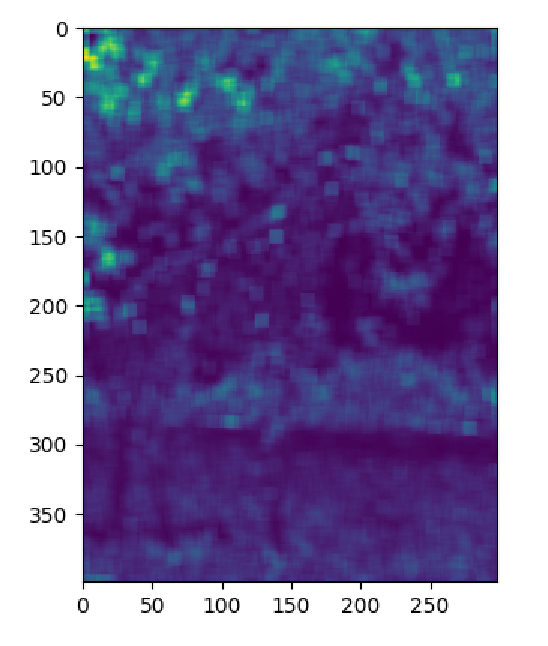
\includegraphics[width=\textwidth]{Bilder/MSE_Bilder/cropped/kernel10_positional_16_0.003_m0_G.eps}
% %     \caption{PE}
% %     \label{MSE16PE}
% %   \end{subfigure}\hfil
% %   \begin{subfigure}{.25\textwidth}
% %     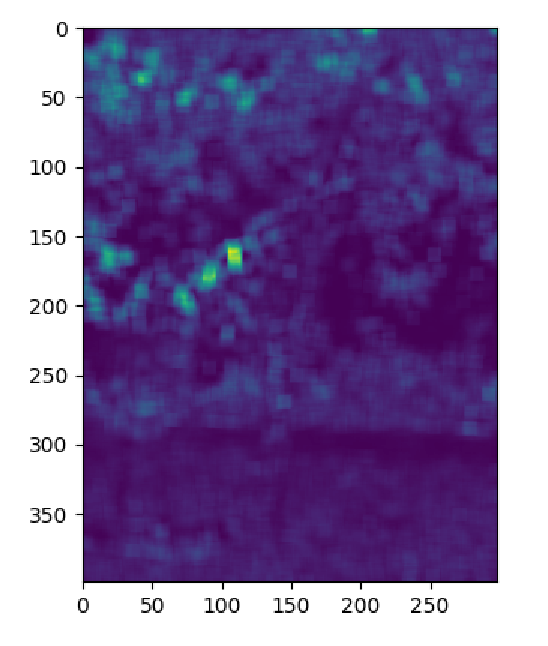
\includegraphics[width=\textwidth]{Bilder/MSE_Bilder/cropped/kernel10_fourier_16_0.01_G.eps}
% %     \caption{FFM}
% %     \label{MSE16FFM}
% %   \end{subfigure}\hfil
% %   \begin{subfigure}{.25\textwidth}
% %     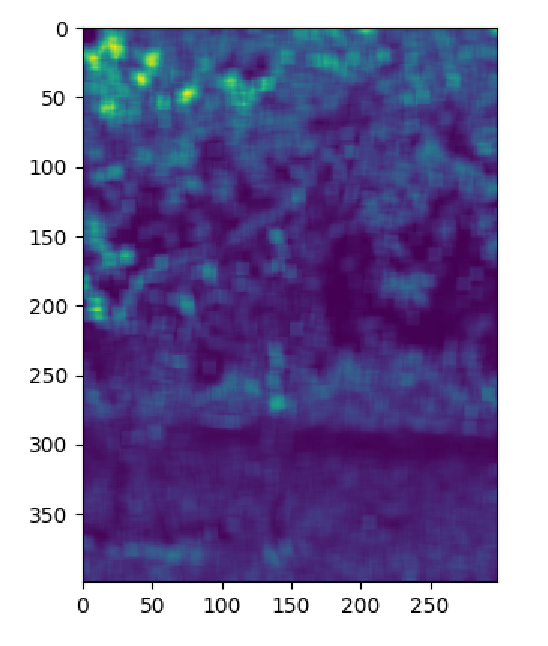
\includegraphics[width=\textwidth]{Bilder/MSE_Bilder/cropped/kernel10_tent16_m4_0.00667_G.eps}
% %     \caption{TE}
% %     \label{MSE16TE}
% %   \end{subfigure}\hfil
% %   \begin{subfigure}{.25\textwidth}
% %     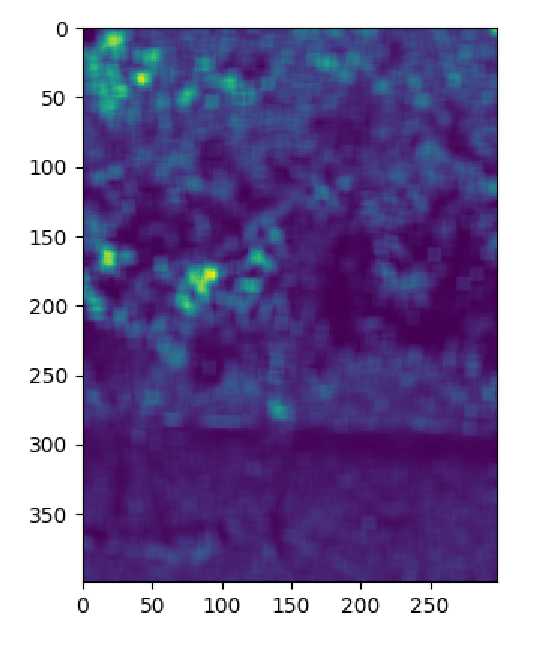
\includegraphics[width=\textwidth]{Bilder/MSE_Bilder/cropped/kernel10_magnitude_16_0.007_m0.05_G.eps}
% %     \caption{ME}
% %     \label{MSE16ME}
% %   \end{subfigure}\hfill
% %   \caption{Local MSE-Loss for $d=16$, green channel, brighter colors represent larger values}
% %   \label{MSE16}
% % \end{figure}

% While each of the encoding approaches leads to better image reconstruction than no enconding at all. The image background exhibits a higher loss than objects in the foreground. This may be attributed to the background features having higher entropy, i.e. higher information content. Another explanation is the occurrence of higher frequency features. PE and FFM lead to better resulting images than TE and ME.

% \begin{figure}
%   \begin{subfigure}{.25\textwidth}
%     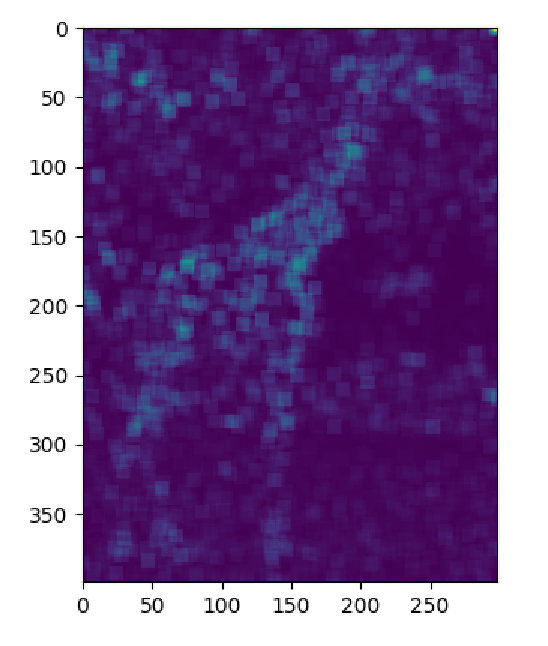
\includegraphics[width=\textwidth]{Bilder/MSE_Bilder/cropped/kernel10_positional_256_0.003_m0_G.eps}
%     \caption{PE}
%     \label{MSE256PE}
%   \end{subfigure}\hfil
%   \begin{subfigure}{.25\textwidth}
%     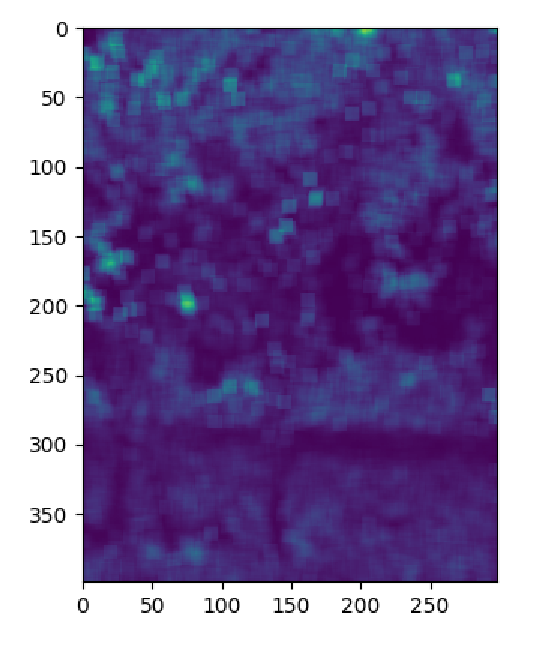
\includegraphics[width=\textwidth]{Bilder/MSE_Bilder/cropped/kernel10_fourier_256_0.01_G.eps}
%     \caption{FFM}
%     \label{MSE256FFM}
%   \end{subfigure}\hfil
%   \begin{subfigure}{.25\textwidth}
%     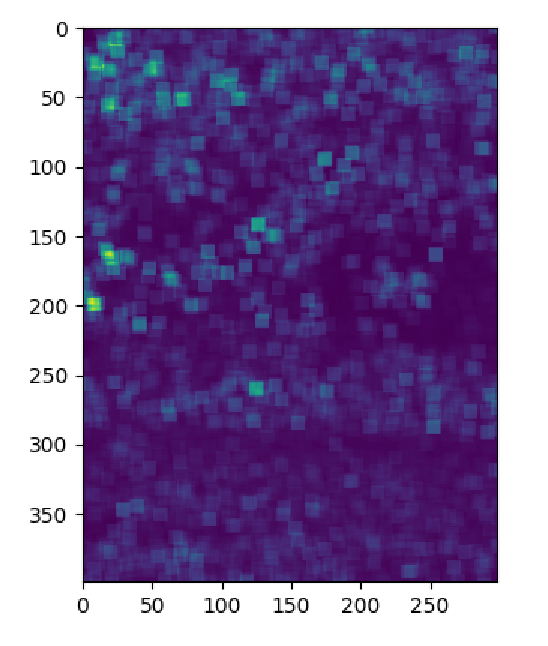
\includegraphics[width=\textwidth]{Bilder/MSE_Bilder/cropped/kernel10_tent_256_0.007_m64_G.eps}
%     \caption{TE}
%     \label{MSE256TE}
%   \end{subfigure}\hfil
%   \begin{subfigure}{.25\textwidth}
%     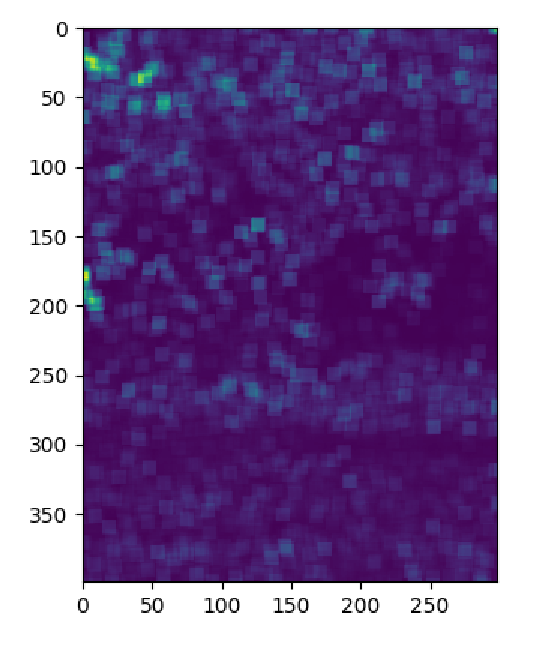
\includegraphics[width=\textwidth]{Bilder/MSE_Bilder/cropped/kernel10_magnitude_256_0.007_m0.0001_G.eps}
%     \caption{ME}
%     \label{MSE256ME}
%   \end{subfigure}\hfill
%   \caption{Local MSE-Loss for $d=256$, green channel, brighter colors represent larger values}
%   \label{MSE256}
% \end{figure}

% In the loss map for PE with $d=256$ the giraffe stands out. This can be attributed to the encoding losing resemblance in the neighborhood of each pixel. This can be interpreted as the encodings of neighboring coordinates lacking similarity which impedes generalization. Training pixels are unaffected by this problem causing the model to overfit.